\documentclass[twocolumn, 10pt]{asme2ej}
\usepackage{epsfig}
\usepackage{hyperref}
\usepackage{graphicx}
\graphicspath{ {images/} }
\usepackage{multirow}
\usepackage{array}
\usepackage{subcaption}

\title{Artifice: Generalized Object Detection in Laboratory Images}

\author{Benjamin Killeen
  \affiliation{
    \href{mailto:killeen@uchicago.edu}{killeen@uchicago.edu}
  }
}

\author{Gordon Kindlmann \affiliation{
    \href{mailto:glk@uchicago.edu}{glk@uchicago.edu}
  }
}

\begin{document}
\maketitle

\begin{abstract}
  {\it Together with large training sets, Deep Neural Networks (DNNs) have
    enabled a wide range of advancements in Computer Vision tasks, especially
    with regard to object detection in real-world images. Object detection for
    laboratory images, on the other hand, presents challenges unlike more
    traditional vision tasks. First, experiments exhibit a scarcity of labelled
    data, a problem which we address through active learning and data
    augmentation. Second, scientific experiments involve inherent constraints,
    such as a natural law or governing principle, which the experimenter intends
    to observe. Although this quality seems advantageous for data augmentation,
    it threatens to undermine the scientific rigor of DNNs for laboratory
    tasks. In this progress report, we describe our ongoing effort toward
    training and verification of DNNs which are agnostic to inherent constraints
    while.}
\end{abstract}

\section{Introduction}
\label{sec:introduction}

Recent advances in compute power have allowed neural networks to grow in both
size and complexity, tackling increasingly sophisticated tasks with applications
including facial recognition and self-driving. However, this success relies on
the availability of very large, well-labeled datasets like ImageNet
\cite{deng_imagenet:_nodate} or COCO \cite{lin_microsoft_2014}, which facilitate
supervised training. Although ``real-world'' applications 

\section{Method}
\label{sec:method}

\begin{figure*}
  \centering
  \begin{subfigure}{0.4\linewidth}
    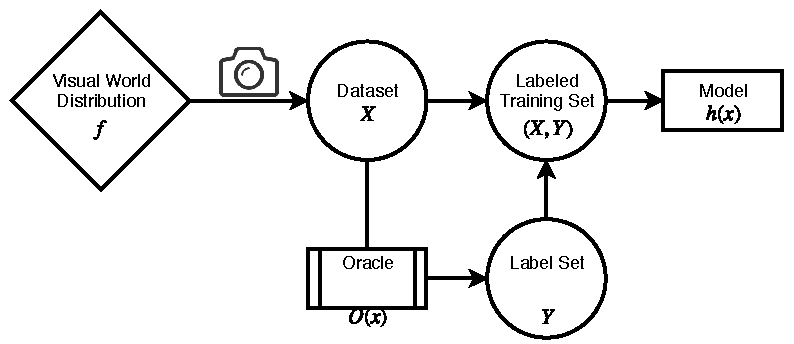
\includegraphics[width=\columnwidth]{traditional_graph}
    \caption{Traditional dependency graph}
    \label{fig:general-graph}
  \end{subfigure}
  \hspace{0.1\linewidth}
  \begin{subfigure}{0.4\linewidth}
    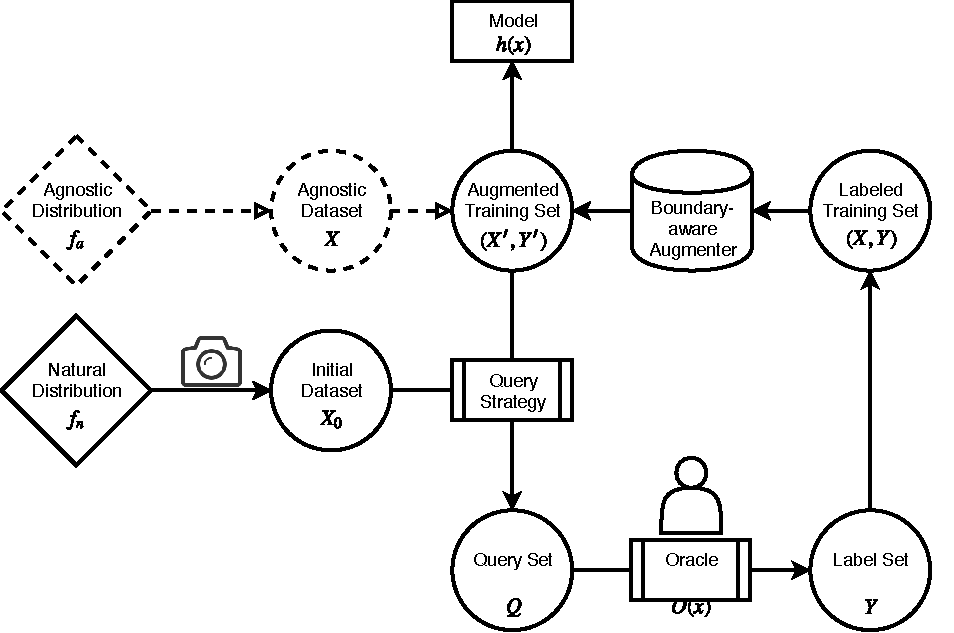
\includegraphics[width=\columnwidth]{artifice_graph}
    \caption{Artifice's dependency graph}
    \label{fig:artifice-graph}
  \end{subfigure}
  \caption{For a traditional vision task (\textbf{a}), a camera converts
    real-world \textit{scenes} into an unlabeled dataset $X$. These scenes have
    actual attributes $\tilde{Y}$ which a \textit{labeller} records as the
    ``ground truth'' or ``measurement'' $Y$. A classifier or regression model
    $f$, trained on $(X,Y)$, produces predictions $\hat{Y}$.\\
    Artifice's dependency graph (\textbf{b}), specialized for object detection
    in laboratory images, distinguishes between two types of
    constraints. \textit{Imposed constraints}, such as physical boundaries, are
    known to the experimenter, but \textit{inherent constraints}, such as a
    physical law, are the subject of hypothesis. \textit{Adverse noise},
    including lighting changes or object deformation, also influences the
    experiment. In (\textbf{b}), the augmented dataset $X$ is continually
    updated by the Training Cycle. A \textit{selector} chooses the query set
    $Q \subseteq X'$ based on existing predictions $\hat{Y}$. A \textit{labeler}
    produces imperfect ground truth $Y$, which enables the \textit{augmenter} to
    intelligently update the dataset $X'$, incorporating imposed
    constraints. Here, dashed lines represent single instance connections, such
    as instantiating $X' \gets X$, rather than continual dependency throughout
    the Training Cycle.}
  \label{fig:dependency-graphs}
\end{figure*}

\bibliographystyle{asmems4}
\bibliography{artifice}

\end{document}
%%% Local Variables:
%%% mode: latex
%%% TeX-master: t
%%% End:
